\documentclass[12pt,fleqn]{article}\usepackage{../../common}
\begin{document}
Dinamik Programlama

Dinamik programlamanın (DP) temelinde ardı ardına verilen kararların
bulunması / hesaplanması fikri vardır; ilgilendiği problemler her verilen
kararın diğer karar seçeneklerini ortaya çıkardığı türden problemlerdir, ve
her seferinde bu seçeneklerin arasından bir tanesi seçilmelidir. Amaç en
iyi karar zincirini bulmaktır. Metot olarak kullanılanlar kısmen ``açgözlü
algoritmalar (greedy algorithms)'' olarak bilinen algoritmaların yaptığına
benzer fakat açgözlü algoritmalar en kısa yolu bulmaya uğraşırken, gezilen
düğümlerde sadece ``o an için'' en iyi seçimi yapar. Bu tür seçim nihai
sonuç göze alındığı zamanen iyi sonucu vermeyebilir. Alttaki grafiğe
bakarsak,

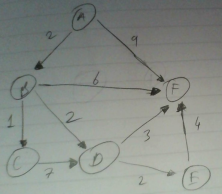
\includegraphics[height=6cm]{dp1.png}

diyelim ki \verb!a! noktasından \verb!f! noktasına en kısa yoldan ulaşmaya
çalışıyoruz - açgözlü algoritma \verb!a,b,c,d! üzerinden gidiş yapardı
çünkü her an, sadece o an için en iyi olanı seçerdi. Fakat en iyi yol
\verb!a,b,d! üzerinden giden yoldur. Gösterilen çizit / ağ yapısı (graph)
yönlü ve çevrimsiz (directed, acyclic graph -DAG-) olarak bilinen bir
yapı. Tipik kısa yol problemleri bu yapılar üzerinde çalışırlar.

DP problemleri özellikle bir problemi alt problemlere bölebildiğimiz zaman
faydalıdırlar, ve bu alt problemler tekrar tekrar hesaplanıyorlarsa da bu
daha iyidir, çünkü DP o alt problemleri önbellekleyerek (caching) tekrar
hesaplanmadan geri getirilmelerini sağlayabilir. 

Üstteki en kısa yol problemini DP ile çözelim.

Önce bazı teorik, mantıksal konular: tümevarımsal olarak düşünelim. Diyelim
ki üstteki DAG'de $a,f$ arasındaki en kısa yolu kesinlikle
``biliyoruz''. Ve yine diyelim ki bu yol üzerinde / bir ara nokta $x$
noktası var. O zaman, $a,x$, ve $x,f$ arasındaki yollar da tanım itibariyle
en kısadır. İspatlayalım: eğer mesela $x,f$ arasındaki en kısa yol
bildiğimizden {\em başka} olsaydı, o zaman eldekini atıp o yolu kullanıyor
olurduk (en kısa olduğunu kesin biliyoruz ya), ve bu sefer o alternatif en
kısa olurdu. Fakat ilk başta en kısa yolu bildiğimiz faraziyesi ile
başladık. Bir çelişki elde ettik, demek ki ara noktanın kısalığı doğrudur
$\square$

Bu ispattan hareketle kısa yolu tek sayısal (numeric) bir değer olarak
hesaplamaya uğraşabiliriz.

Öyle bir fonksiyon $d(v)$ olsun ki herhangi bir $v$ nodu için o nod'dan
bitiş noktasına olan en kısa uzaklığı kesin biliyor olsun (dikkat, bu
hesabın nasıl olacağını düşünmüyoruz şimdilik, sadece olabileceğini, olmuş
olduğunu farz ediyoruz). Çoğu tümevarımsal tasarımda olduğu gibi hesabın
kendisinin özyinelilik (recursive) çağrı zincirinin mekaniği içinde
halolmasını amaçlıyoruz. Doğru olan bir ifadeyi düşünüyoruz öncelikle, ve
hesabın kendisini sürekli bir sonraki noktaya erteliyoruz. 

Devam edelim: $u,v$ arasındaki parça mesafeler $w(u,v)$'dir. Şimdi, eğer
bir ara nokta $u$'ya gelmişsek -yine tümevarımsal olarak düşünmeye devam
ediyoruz- bu noktanın her komşusu $w$ için $d(w)$'yi ``bildiğimize'' göre,
en kısa yol için tek yapmamız gereken her seçim anında en minimal $w(u,v) +
d(v)$'yi  $u$'nun uzaklığı olarak almaktır.

Veri yapısı olarak DAG'ı alttaki gibi gösterelim,

\begin{minted}[fontsize=\footnotesize]{python}
DAG = {
    'a': {'b':2, 'f': 9},
    'b': {'d':2, 'c':1, 'f': 6},
    'c': {'d':7},
    'd': {'e':2, 'f': 3},
    'e': {'f':4},
    'f': {}
}
\end{minted}

Böylece $w(u,v)$ basit bir Python sözlük (dictionary) erişimi haline
geliyor, \verb!a,b! arası parça mesafe için 

\begin{minted}[fontsize=\footnotesize]{python}
print DAG['a']['b']
\end{minted}

\begin{verbatim}
2
\end{verbatim}

En kısa yolu bulacak program

\inputminted[fontsize=\footnotesize]{python}{memo.py}

\begin{minted}[fontsize=\footnotesize]{python}
from memo import *

def rec_dag_sp(W, s, t): 
    @memo                                    
    def d(u):
        print 'Dugum:' + u[0]
        if u == t:  print 'Son nokta t, geri donus'; return 0  
        min_dist = min(W[u][v]+d(v) for v in W[u])  
        print 'Geri donus,',u,'uzerindeyiz, mesafe=',min_dist
        return min_dist
    return d(s)                                 

dist = rec_dag_sp(DAG, 'a', 'f')
print 'toplam mesafe=', dist
\end{minted}

\begin{verbatim}
onbellekte yok - a
Dugum:a
onbellekte yok - b
Dugum:b
onbellekte yok - c
Dugum:c
onbellekte yok - d
Dugum:d
onbellekte yok - e
Dugum:e
onbellekte yok - f
Dugum:f
Son nokta t, geri donus
Geri donus, e uzerindeyiz, mesafe= 4
onbellekte var - f
Geri donus, d uzerindeyiz, mesafe= 3
Geri donus, c uzerindeyiz, mesafe= 10
onbellekte var - d
onbellekte var - f
Geri donus, b uzerindeyiz, mesafe= 5
onbellekte var - f
Geri donus, a uzerindeyiz, mesafe= 7
toplam mesafe= 7
\end{verbatim}

Şimdi çağrı mekaniğinin hakikaten nasıl işlediğini görelim. Not: Önbellek
kodlaması dekoratör kullanıyor, dekoratörler hakkında bir yazı için [2].

Başlangıç $u$, oradan, minimum seçerken, sürekli $d()$ çağrısı yapıyoruz,
yani $d()$ kendini çağırıyor. Çağrının geri dönmesinin tek yolu son noktaya
erişmek. Bu ne demektir? Programımız daha hesap yapmadan ``derinliğine bir
dalış'' yapıyor. Son noktalara gelene kadar özyineli çağrıları ardı ardına
uyguluyor, esas hesapları geri dönüş sırasında yapıyor. Bu nasıl ise
yarıyor? Ayrıca önbelleklemenin hakikaten işleyip işlemediğini nasıl
bileceğiz?  Ya da önbellekteki bir değerin hep en iyisi olduğunu nereden
bileceğim? 

Bu arada, böyle bir yaklaşımda, önbellek değeri bir kez set edildi mi,
hiç değiştirmeye gerek yok.

Nokta \verb!d!'ye bakalım. Bu noktanın mesafesi (yani son nokta \verb!f!'ye
uzaklığı) kararlaştırılırken algoritma \verb!d!'nin her komşusuna
bakacaktır, bunu \verb!for v in W[u])! ile yapacaktır. Her komşu için
\verb!f!'ye gelene kadar o yol derinliğine takıp edilecektir. Üstteki
çıktıda görüyoruz ki \verb!d! sonrası iki komşu \verb!e,f! için önce
\verb!d-f! ve \verb!d-e-f! gidişi yapılmıştır (amaç hep o son noktaya
ulaşmak, unutmayalım). 'Komşulara bakma ve aralarından en azı seçme''
mantığı tüm bu yollar denenene kadar bekleyecektir, ancak hepsi bittikten
sonra içlerinden bir minimum seçecektir.

İşte şimdi niye her düğümdeki minimum hesabının en iyisi olduğunu
anlıyoruz, çünkü o noktadan nihai noktaya varış için tüm alternatifler
deneniyor. O derine dalışın sonuçları arasından bir tanesi
seçiliyor. önbellekteki değer bu sebeple bir kez set ediliyor, ve hiç
değişmiyor. Tabii ki önbellekteki değer tekrar tekrar kullanılabiliyor,
\verb!c!  için bir \verb!d! uzaklığı gerektiğinde bu önbellekten servis
edilecektir.

Ve her düğümdeki minimum hesabı en iyiyse, bu hesapları kullanan başlangıca
yakın noktaların hesabı da doğal olarak en iyisi (kısası) olacaktır. Başta
tümevarımsal olarak belirttiğimizin tekrar ifade edilmesidir bu. 

Kısa Yol Tarifini Bulmak

Mesafe hesabı işte böyle yapılıyor... Peki en kısa yolun kendisini nasıl
biliriz? Yani önce şuraya, sonra şuraya git türünden yol tarifi bilgisi
nasıl hesaplanır? Aslında komşular arasındaki en kısa mesafeyi seçme
problemi, o komşular içinden hangisinin o en mesafeyi sağladığını hatırlama
problemine oldukça benziyor. Yani, her düğüm üzerindeyken ve komşular
arasından en kısa mesafeyi seçerken, o mesafenin ``hangi komşudan''
geldiğini hatırlamak ve bunu bir yerlere kaydetmek yeterli. Her düğüm için,
son noktaya olan en kısa mesafe değişmediğine göre, ``o mesafe bilgisinin
geldiği komşunun hangisi olduğu'' bilgisi de değişmeyecektir. Ve her nokta
için o ``ebeveyn komşu'' bilindiği zaman herşey işleyip bittikten sonra en
kısa yol tarifi için eldeki kayda bakarız, ve başlangıç noktası
\verb!a!'dan başlayarak zıplaya zıplaya o ebeveyn zinciri ile sona kadar
geliriz. Bu değişiklikleri ekleyince kod şu hale gelir,

\inputminted[fontsize=\footnotesize]{python}{sp.py}

\begin{minted}[fontsize=\footnotesize]{python}
import sp
dist, parent = sp.rec_dag_sp2(DAG, 'a', 'f')
print 'ebeveynler', parent
\end{minted}

\begin{verbatim}
onbellekte yok - a
onbellekte yok - b
onbellekte yok - c
onbellekte yok - d
onbellekte yok - e
onbellekte yok - f
Geri donus, e uzerindeyiz, mesafe= 4
onbellekte var - f
Geri donus, d uzerindeyiz, mesafe= 3
Geri donus, c uzerindeyiz, mesafe= 10
onbellekte var - d
onbellekte var - f
Geri donus, b uzerindeyiz, mesafe= 5
onbellekte var - f
Geri donus, a uzerindeyiz, mesafe= 7
ebeveynler {'a': 'b', 'c': 'd', 'b': 'd', 'e': 'f', 'd': 'f'}
\end{verbatim}

Not: \verb!argmin! bir liste içindeki en minimal değerin indisini verir. 

İşte sonuç. Başlangıç \verb!a!, onun ebeveyni \verb!b!. \verb!b!'ye
bakıyoruz, onunki \verb!d!. Oradan \verb!f!'ye atlıyoruz, ve sonuca erişmiş
oluyoruz, en kısa yol \verb!a-b-d-f!. 

Analiz

Açgözlü yaklaşımdan bu yaklaşımın farkını şimdi daha iyi görebiliriz,
açgözlü teknik her düğümde en azı bizzat takip eder, ve kısayol hesabı,
mesafe hesabı hep bu takip eylemi sırasın o anda yapılır, elde bir toplam
vardır ve ona eklenir, vs. Bu yaklaşım daha hangi yolu seçtiği, sonradan,
birkaç adım sonrasında hiçbir seçimle ilgilenmez. Dinamik Programlama ise
takip etme eylemi ile hesap eylemini birbirinden ayırır, ve tümevarımsal
bir tanımdan yola çıkarak, hep en kısa, en optimali bulmayı başarır.

DP algoritmasının karmaşıklığı, $M$ tane bağlantı (edges) ve $N$ tane düğüm
için $O(N + M)$'dir. Yani çözüm lineer zamandadır! Alt problemleri tekrar
tekrar çözüyoruz evet, ve \verb!@memo! ibaresini koddan çıkartsaydık
algoritmamızın üstel (exponential) zamanda işlediğini görürdük, ki bu çok
kötüdür. Fakat çözülen alt problemleri bir daha çözmeyip sonuçlarını
önbellekten aldığımız için algoritma son derece hızlı işliyor.

Kaynaklar

[1] Hetland, M., L., {\em Python Algorithms, 8. Bolum}

[2] Bayramlı, {\em Dekoratorler, Onbellek Kodlamasi, Fonksiyon Degistirmek}, 
    \url{https://burakbayramli.github.io/dersblog/sk/2013/07/onbelleklemeyi-dekorator-ile-yapmak.html}

\end{document}
